% sage_latex_guidelines.tex V1.20, 14 January 2017

%\documentclass[Afour,sageh,times]{sagej} %IJRR
\documentclass[letterpaper, 10 pt, conference]{ieeeconf} % 
\overrideIEEEmargins
\IEEEoverridecommandlockouts

\usepackage{amsmath}
\usepackage{amscd}  
\usepackage{bm,upgreek}
\usepackage{amsfonts}
\usepackage{wasysym}
\usepackage{amsthm}
\usepackage{amssymb}
\usepackage{nccmath}
\usepackage{epsfig}
\usepackage{moreverb,url}
\usepackage{graphicx}
%\usepackage[font=footnotesize]{caption}
%\usepackage[font=footnotesize]{subcaption}
\usepackage{capt-of}
\usepackage{booktabs}
\usepackage{xcolor}
%\usepackage{citesort}
%\usepackage{accents}
\usepackage{import}
\usepackage{placeins}
\usepackage{mathtools}
%\usepackage{subcaption}
\usepackage{array}
\usepackage{multirow}
\usepackage{tabu}
\usepackage{booktabs}
\usepackage{cite}

\usepackage{transparent}
\pdfminorversion=4

% Track additions
\newcommand*{\ta}[1]{\textcolor[HTML]{107f10}{#1}}
\newcommand*{\tb}[1]{#1}
\newcommand*{\tc}[1]{#1}
\newcommand*{\td}[1]{#1}
\newcommand*{\te}[1]{#1}
\newcommand*{\tf}[1]{#1}

% Track removal
\newcommand*{\ra}[1]{}
\newcommand*{\rb}[1]{}
\newcommand*{\rc}[1]{}
\newcommand*{\rd}[1]{}
\newcommand*{\re}[1]{}
\newcommand*{\rf}[1]{}


% \newcommand*{\TODO}{\textcolor[HTML]{FF0000}{\bf TODO:}}
% \graphicspath{{figs/}{latex/figs/}}

% %\newcommand{\ubar}[1]{\underaccent{\bar}{#1}} %% conflicting defs
\newcommand{\rt}{\textcolor{red}}

% Alter some LaTeX defaults for better treatment of figures:
% See p.105 of "TeX Unbound" for suggested values.
% See pp. 199-200 of Lamport's "LaTeX" book for details.
%   General parameters, for ALL pages:
\renewcommand{\topfraction}{0.9}	% max fraction of floats at top
\renewcommand{\bottomfraction}{0.8}	% max fraction of floats at bottom
%   Parameters for TEXT pages (not float pages):
\setcounter{topnumber}{2}
\setcounter{bottomnumber}{2}
\setcounter{totalnumber}{4}     % 2 may work better
\setcounter{dbltopnumber}{2}    % for 2-column pages
\renewcommand{\dbltopfraction}{0.9}	% fit big float above 2-col. text
\renewcommand{\textfraction}{0.07}	% allow minimal text w. figs
%   Parameters for FLOAT pages (not text pages):
\renewcommand{\floatpagefraction}{0.7}	% require fuller float pages
% N.B.: floatpagefraction MUST be less than topfraction !!
\renewcommand{\dblfloatpagefraction}{0.7}	% require fuller float pages

% remember to use [htp] or [htpb] for placement


\DeclareMathOperator{\Parallel}{Parallel}
\DeclareMathOperator{\Series}{Series}

\DeclareMathOperator{\sign}{sign}
\DeclareMathOperator{\sinc}{sinc}
\DeclareMathOperator{\rank}{rank}
\DeclareMathOperator*{\argmin}{arg\,min}

\newcommand*{\htwo}{\mathcal H_2}
\newcommand*{\hinf}{\mathcal H_\infty}
\newcommand*{\jo}{(j\omega)}
\newcommand*{\s}{(s)}
\newcommand*{\tr}{\mathrm{tr}}
\newcommand*{\AM}{\mathrm{AM}}
\newcommand*{\GM}{\mathrm{GM}}

\pdfsuppresswarningpagegroup=1
\pdfminorversion=4

\newcommand\blfootnote[1]{%
	\begingroup
	\renewcommand\thefootnote{}\footnote{#1}%
	\addtocounter{footnote}{-1}
	\endgroup
}

\theoremstyle{plain}
\newtheorem{theorem}{Theorem}
\newtheorem{proposition}{Proposition}
\newtheorem{conjecture}{Conjecture}
\newtheorem{corollary}{Corollary}[theorem]
\newtheorem{lemma}{Lemma}

% Define roman thorem types
\theoremstyle{definition}
\newtheorem{problem}{Convex Problem}
\newtheorem{definition}{Definition}

% Definie low-key roman thorem types
\theoremstyle{remark}
\newtheorem{remark}[theorem]{Remark}

\newenvironment{leveldown}% Demote sectional commands
{   \let\chapter\section%
	\let\section\subsection%
	\let\subsection\subsubsection%
	\let\subsubsection\paragraph%
	%\let\subparagraph\relax%
}{}

%\newtheorem{definition}{Definition}
\newcommand{\underbracedmatrix}[2]{%
	\left(
	\smash[b]{\underbrace{
			\begin{matrix}#1\end{matrix}
		}_{#2}}
	\right)
	\vphantom{\underbrace{\begin{matrix}#1\end{matrix}}_{#2}}
}
\newcommand{\minimatrix}[1]{\mbox{\tiny $\setlength{\arraycolsep}{2pt}\begin{pmatrix} #1 \end{pmatrix}$}}

\newcommand{\noop}[1]{}
\newcommand{\link}[2]{{\bf\color{blue}\underline{\smash{#2}}}}

% \newcommand\BibTeX{{\rmfamily B\kern-.05em \textsc{i\kern-.025em b}\kern-.08em
% T\kern-.1667em\lower.7ex\hbox{E}\kern-.125emX}}

% \def\volumeyear{2021}
% \setcounter{secnumdepth}{3} % numbers sections


% \title{A Lightweight Rotary Spring Design}
\title{\LARGE \bf A Compact, Two-Part Torsion Spring Architecture}

\author{Zachary Bons$^{1,2}$, Gray C. Thomas$^{1,3}$, Luke M. Mooney$^{4}$ and Elliott J. Rouse$^{1,2,3}$% <-this % stops a space
\thanks{$^{1}$ Neurobionics Lab, University of Michigan, Ann Arbor, USA}%
\thanks{$^{2}$ Department of Mechanical Engineering, University of Michigan, Ann Arbor, USA {\tt\small \{zbons, ejrouse\}@umich.edu}}%
\thanks{$^{3}$ Department of Robotics, University of Michigan, Ann Arbor, USA}%
\thanks{$^{4}$ Dephy Inc., Maynard, MA, USA}%
\thanks{This work was supported by the National Science Foundation National Robotics Initiative under Grant 2024237 and Grant 1830338.}%
\thanks{Digital Object Identifier XX.XXXX/SRO.2022.XXXXXXX}
}


\begin{document}


\maketitle
\thispagestyle{empty}
\pagestyle{empty}

\begin{abstract}
Springs are essential mechanical elements that are used across a wide variety of industries and mechanisms...
\end{abstract}

% Note that keywords are not normally used for peer review papers.
% \begin{IEEEkeywords}
% 	Spring, Series Elastic Actuators, Robotics.
% \end{IEEEkeywords}

\section{INTRODUCTION} \label{sec:intro}
Springs are among the most ubiquitous and important mechanical elements used in robotic systems. A key functionality enabled by springs is the ability to sense the force or torque applied by an actuator. This functionality is exploited when elastic elements are applied between the output of the transmission and the load, a configuration known as a Series-Elastic Actuator (SEA) \cite{PrattWilliamson1995IROS}. SEAs gained popularity due to their improved force/torque fidelity, energy storage, and shock tolerance. Their compliant nature has been used extensively in human-centric applications \cite{Pratt2002IR,FitzgeraldBaxter2013,KongBaeTomizuka2009TMech,ShepherdRouseExo2017}, where a low-impedance interaction at the robot interface is often desirable. Despite drawbacks of SEAs---namely a reduction in force bandwidth and increased mass and complexity---they have driven substantial development of rotary spring designs. Increasing energy storage per unit mass (specific energy) and volume (energy density) has been a key focus of these innovations.

The geometry of different springs is one of the most important aspects of their design. In wearable or legged robots, torsion springs are often more advantageous due to the inherent rotary nature of their architectures. Elastic elements like simple torsion springs, including tubes \cite{Williamson1999Dissertation,Pratt2002ICB} and cantilevers with cam-rollers \cite{ShepherdRouse2017} or hinges \cite{HubickiGrimes2016} are often impractical due to their size and/or mass. Consequently, researchers have focused on planar, disk-like designs that consist of a central anchor point connected to a rigid outer rim via a set of flexible elements, known as \textit{flexures}. Relative motion between the anchor point and rim loads the flexures and spring-like behavior is achieved. The most prominent planar torsion spring geometry is comprised of spiral flexure arms that extend from the central anchor to the rim \cite{KnoxSchmiedeler2009JMD,Stienen2010TBME,LagodaEA2010ICBRB,WangMeijnekeVanderkooij2013ICORR,GeorgievBurdick2017IROS,YooChungMech2017}. These springs have enabled many advancements, can achieve high energy density, and have seen many promising uses in robotic systems \cite{WangVanderkooij2015NSRE,Chaichaowarat2018EMBS,PaineOhSentis2014TMech,BrownNesnas2018IROS}. However, by constraining the spiral arms on both ends of the flexure, these springs constrain the strain rate, requiring that the slope of the strain as a function of radius be continuous. Ultimately, this constraint limits the potential deflection. In addition, spiral designs can cause significant directional differences in stiffness profile \cite{YooChungMech2017}. A variety of unique flexure designs have been explored with the principal objective of high torque-sensing resolution \cite{CarpinoEA2012JMD,PaineEA2015JFR,AccotoEA2013IJARS,DossantosCurinSiqueira2017CEP,KimKong2021,FioreziAndrade2020,CummingsSup2016}, but these approaches have generally further reduced the allowable range of motion and maximum torque. Thus, there remains a gap in the development of compact torsion springs with larger deflections and symmetric stiffness profiles.  

A second key design attribute is the spring's loading condition during use, as it greatly impacts both the spring's energy density and specific energy. Specifically, certain loading conditions impose strict limits on the amount of energy that can be stored within a material. For example, pure tension loads all elements of a beam equally, resulting in maximal energy storage per mass; however, pure torsion of a solid rod loads the outer edge of the material optimally, but induces little to no strain at the center, resulting in comparatively low energy storage. While monolith-style spring designs have proven effective in several performance measures, they are limited in energy storage by the inefficiency of bending elements that are fully fixed at both ends. Balancing favorable loading conditions and simplicity of spring assembly, Herodotou \textit{et al.} conceived a spring design defined using a spiral flexure that is fixed at one end and hinged at the other \cite{HerodotouWang2019ICORR}. The physical spring closely matched modeled behavior, but the analysis showed only springs with high stiffness (1950 Nm/rad) and did not yet indicate scalability to lower stiffness regimes.
\begin{figure}[h!]
    \centering
    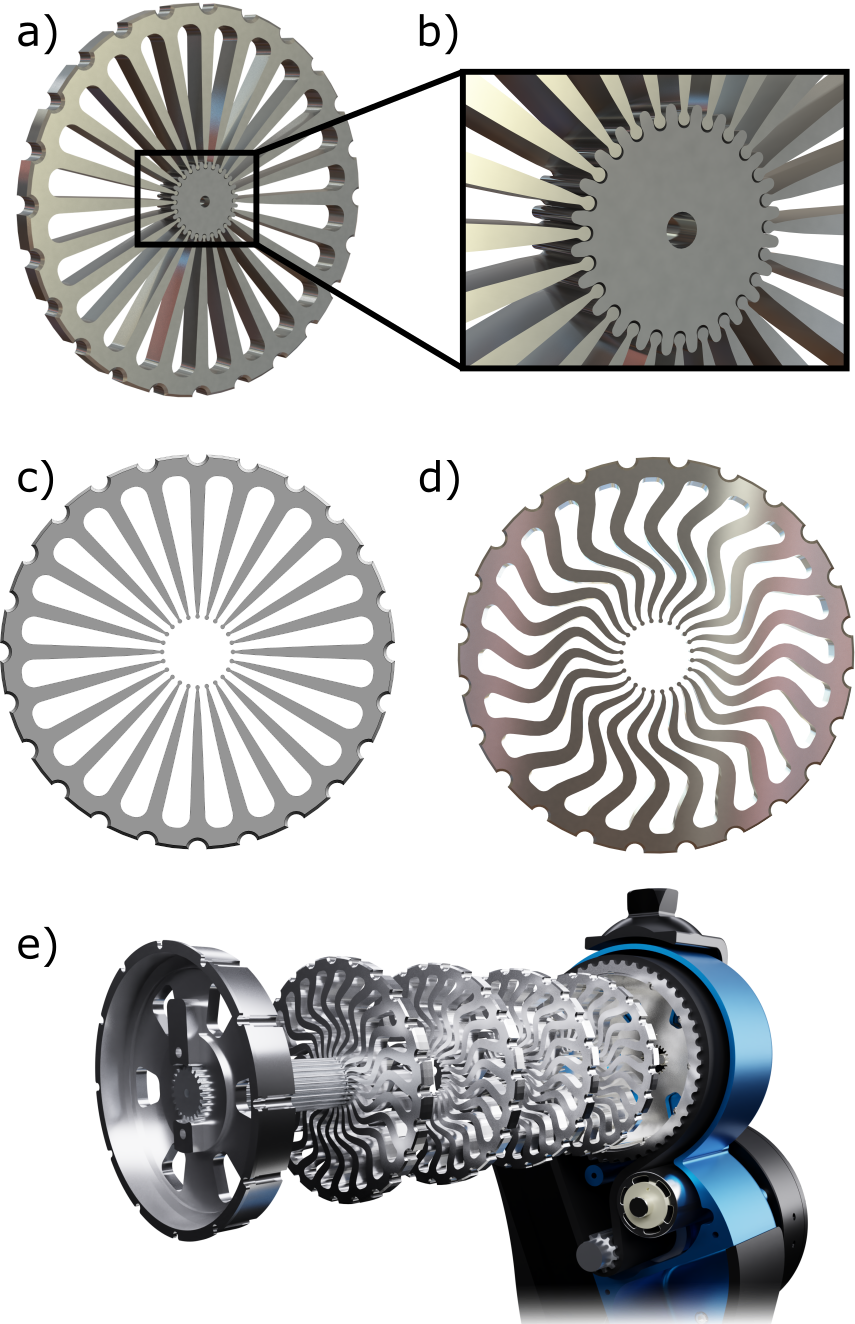
\includegraphics[width=\columnwidth]{figs/spring_collage_icra3.png}
    \caption{Rotary spring design based on bending cantilever flexures. a) the original design consists of straight flexures with a tapered profile. b) the flexures mate with a gear-like camshaft, which loads the spring when rotated. c) a planar view of the spring with straight flexures. d) serpentine flexures can be used to increase the energy density of the spring. e) the spring neatly mates with transmission components---in this case, a timing belt pulley in the Open-Source Leg \cite{AzocarRouse2020}.}
    \label{fig:main_design}
\end{figure}
In this paper, we introduce the design framework for a torsion spring architecture and we empirically validate the framework with two representative spring designs. Our spring architecture is motivated by the need to create low stiffness torsion springs in compact designs, and combines convenient geometry with an efficient loading condition to yield high specific energy and energy density. The springs introduced in this work were inspired by Ref.~\cite{MooneyPaschDoan2017Patent}, and are included within the design of our open-source robotic leg prosthesis \cite{AzocarRouse2020}. Notably, they were incorporated within the volume of existing components, enabling the function of series-elasticity without increasing size.

\section{SPRING DESIGN}

In this section we introduce our design approach and provide the equations that govern the spring mechanics and geometry. Our intent is to clarify our modeling decisions made within this framework and to give other researchers a detailed understanding needed to modify our approach for their own custom applications.


% \begin{figure}[b!]
%     \centering
%     \includegraphics[width=\columnwidth]{latex_ICRA/figs/spring_collage_icra.png}
%     \caption{Rotary spring design based on bending cantilever flexures. a) the original design consists of straight flexures with a tapered profile. b) the flexures mate with a gear-like camshaft, which loads the spring when rotated. c) the spring neatly mates with transmission components---in this case, a timing belt pulley in the Open-Source Leg \cite{AzocarRouse2020}. d) serpentine flexures can be used to increase the energy density of the spring.}
%     \label{fig:main_design}
% \end{figure}

Our spring design comprises a gear-like camshaft that interfaces with a ring of radially-spaced cantilevered flexures (Fig.~\ref{fig:main_design}). The flexures are joined on the outer edge by a shared ring, which can be constrained inside a housing part using dowel rods (Fig.~\ref{fig:main_design}e). When the camshaft rotates, a force is applied at each flexure tip, causing the flexure to deflect like a cantilever beam as the flexure tip slides along the cam tooth (Fig.~\ref{fig:spring_diag}a). The camshaft is specifically designed to ensure that the flexures do not skip teeth within the allowable range of motion and to result in a force that is perpendicular to the nominal straight flexure. This sliding perpendicular force is key to the cam-flexure interface, as it approximates a pure bending moment and thus ideal bending of the flexure, which is the most energy-efficient loading condition for bending beams. Thus, a key difference in our approach is to design the torsion spring in two parts that can rotate relative to one another; this design eliminates the constraint on the strain rate of the flexures (that is, the slope of the strain as a function of radius can be discontinuous).
\subsection{Straight Tapered Flexures}
By utilizing tapered flexures, the design achieves maximum specific energy. The tapering law \cite{ShepherdRouseExo2017} that governs the flexure geometry enforces equivalent stress along both bending surfaces (Fig.~\ref{fig:spring_diag}b) when the spring is loaded, which allows a significant removal of mass from the uniform (\textit{i.e.} non-tapered) beam. The mathematical expression of the tapering law governs the flexure thickness ($\lambda$) as a function of distance ($x$) along the flexure (Fig.~\ref{fig:spring_diag}b) and is derived from basic mechanics \cite{GoodnoGere2013}.
\begin{figure}[t!]
    \centering
    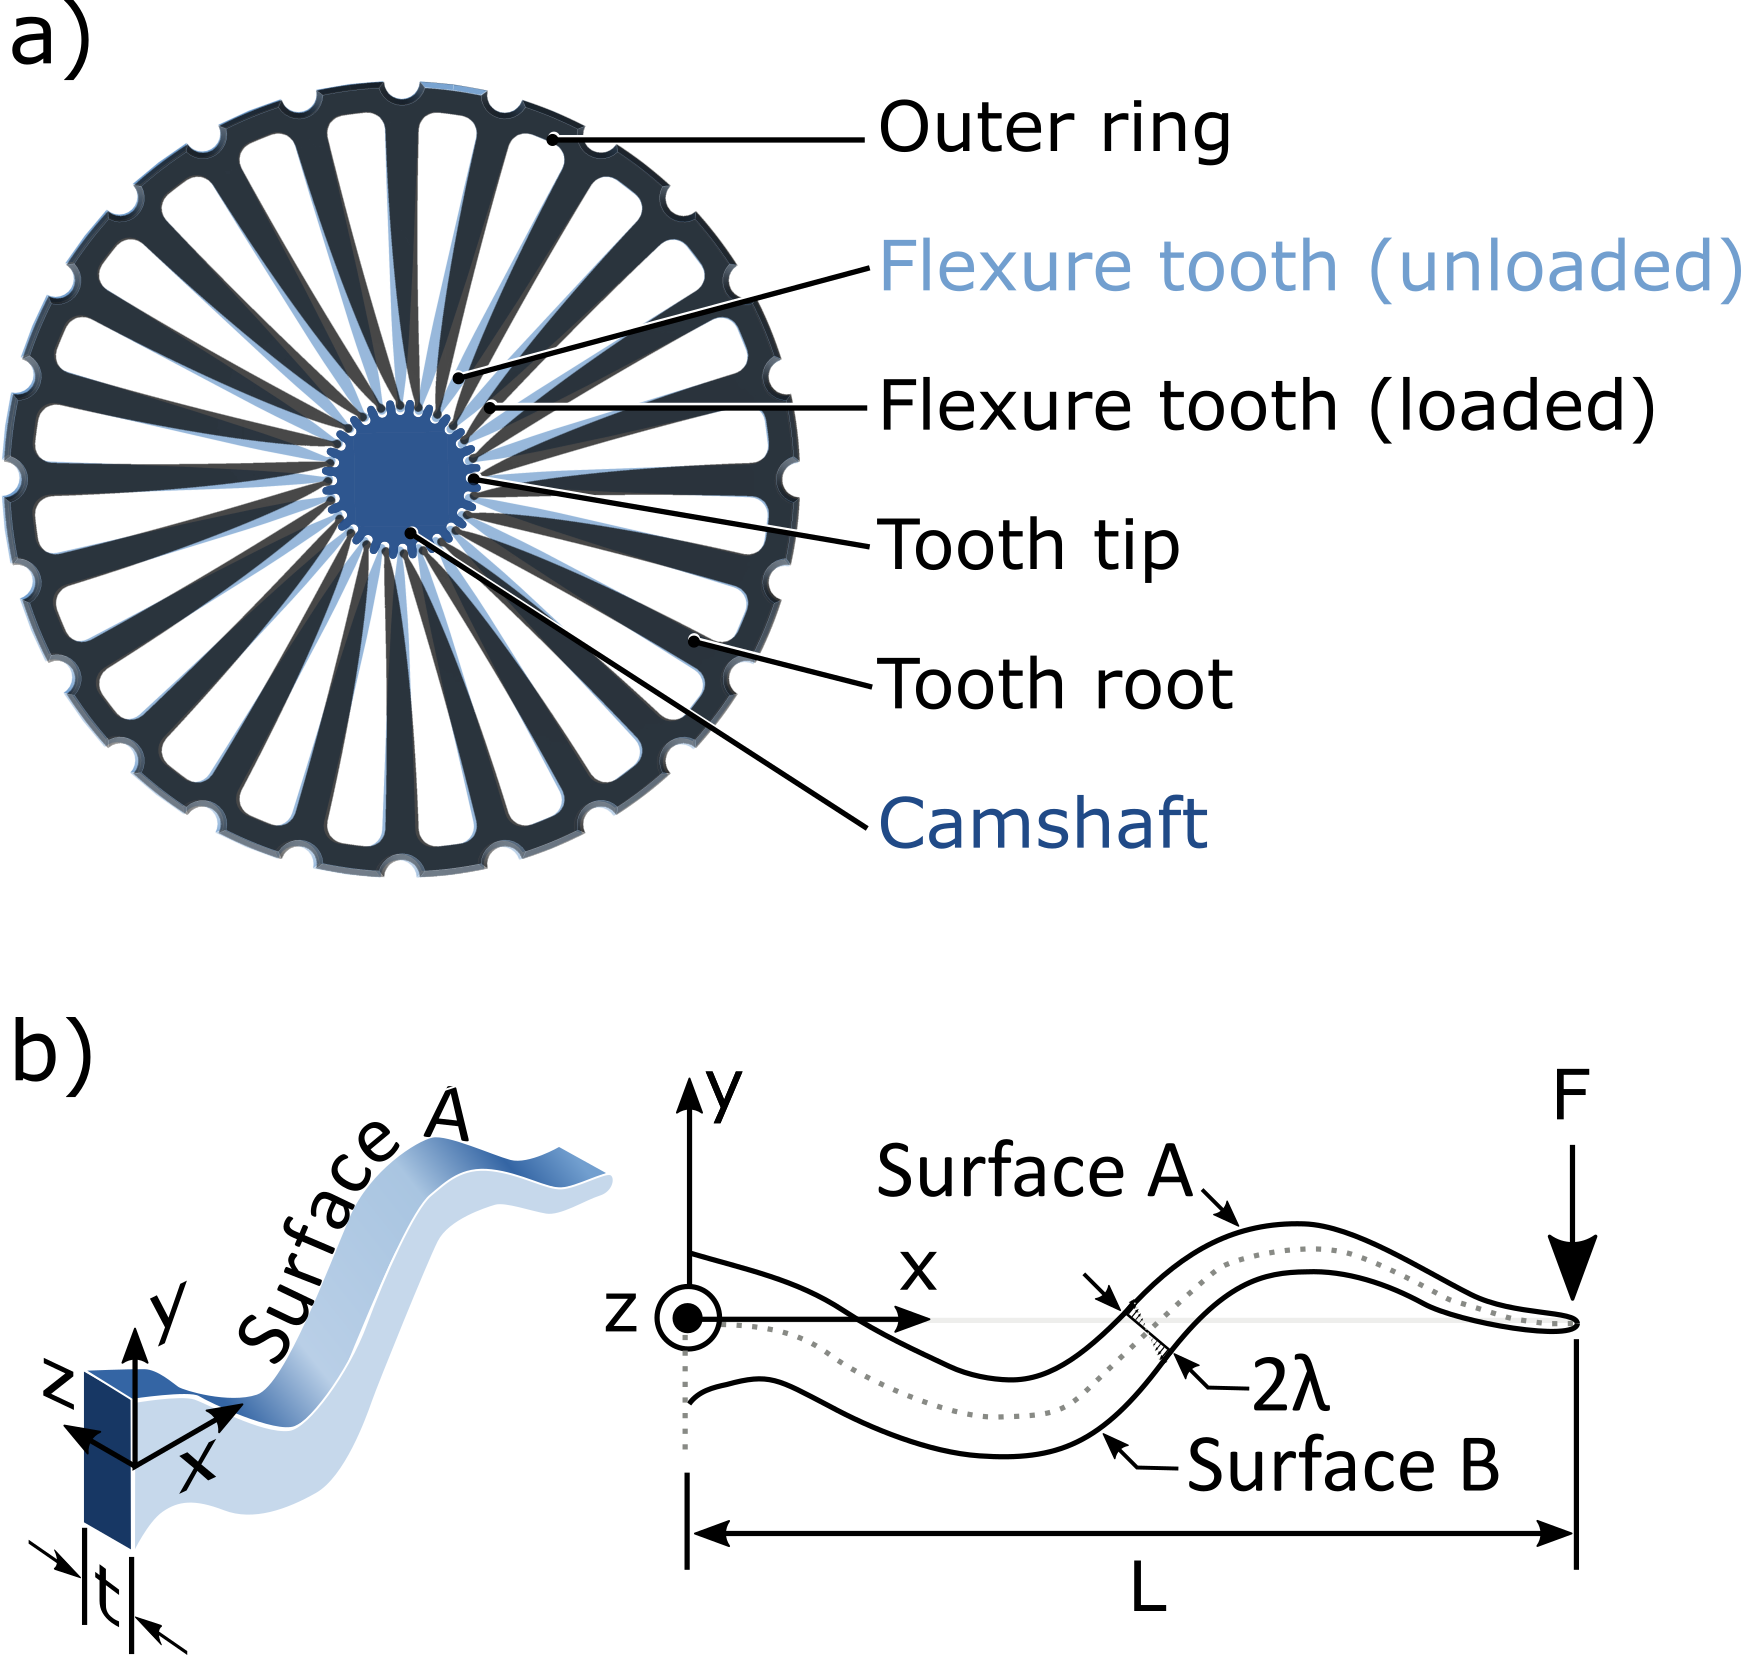
\includegraphics[width=\columnwidth]{figs/spring_diagram.png}
    \caption{a) Straight-flexured spring with labeled features. b) Schematic of beam coordinate frames and loading condition for a serpentine flexure, with surfaces A and B being the bending surfaces. The stated conventions also apply to straight flexures.}
    \label{fig:spring_diag}
\end{figure}
For a generic bending beam, we know that $\sigma = \frac{M\lambda}{I}$, with $\sigma$ as axial stress, $M$ as applied moment ($F(L-x)$ in this case), $\lambda$ as the distance from the neutral axis to the bending surfaces (see Fig.~\ref{fig:spring_diag}b), and $I$ as the second moment of area. Considering our planar spring design, $I = \frac{2t\lambda^3}{3}$, with $t$ as spring thickness (see Fig.~\ref{fig:spring_diag}b). To achieve maximum stress along the beam during maximum loads, we choose $\lambda$ at each $x$ such that $\sigma = \sigma_d$, where $\sigma_d$ is the design stress:

\begin{align}
    \sigma_d &= \frac{3F(L-x)\lambda}{2t\lambda^3}, \\
    \lambda(x) &= \sqrt{\frac{3F(L-x)}{2t\sigma_d}}.
    \label{eqn:flexure_width}
\end{align}

This law fully defines the flexure geometry and can be used to determine a relationship between spring rate and bending strain energy. Equating bending strain energy and desired energy storage of the spring then allows us to predict deflection properties of the spring. This analysis is simplified by three assumptions: first, as mentioned previously, we assume that the camshaft imposes perpendicular forces on the tips of the flexures. Second, the perpendicular force imposes a pure bending moment on the flexure and thus ideal bending occurs at each cross-section of the spring. Lastly, we assume that the spring deflects at only small angles.

With these assumptions in place, we can calculate strain energy as a function of spring parameters. For a generic beam in bending, strain energy ($U$) is defined by $U = \frac{M\theta}{2}$, with $M$ as before and $\theta$ as deflection angle. Furthermore, $\theta = {\kappa}L$, where (curvature) $\kappa = \frac{M}{EI}$. Thus,  $U = \frac{M^2L}{2EI}$. The strain energy of a non-uniform beam can then be written in integral form:
\begin{equation}
    U = \int_{0}^{L} \frac{F^2(L-x)^2}{2EI}\,dx.
\end{equation}
Substituting previous definitions of $I$ and $\lambda$ shows 
\begin{equation}
    U = \int_{0}^{L} \frac{3F^2(L-x)^2}{4Et{\sqrt{\frac{3F(L-x)}{2t\sigma_d}}}^3}\,dx.
\end{equation}
Simplifying,
\begin{equation}
    U = \frac{\sigma_d^2t}{3E}\int_{0}^{L} \sqrt{\frac{3F(L-x)}{2t\sigma_d}}\,dx,
    \label{eqn:prestraightstrain}
\end{equation}
which can be rewritten in closed form as
\begin{equation}
    U = \sqrt{\frac{2tFL^3\sigma_d^3}{27E^2}}.
\end{equation}
Since force ($F$) is a function of stiffness ($k$), deflection ($\theta_{des}$), the number of flexures ($n$) and the flexure-camshaft contact radius ($r$), we appropriately substitute these terms,
\begin{equation}
    U = \sqrt{\frac{2tk{\theta_{des}}L^3\sigma_d^3}{27E^2rn}}.
    \label{eq:straightstrain}
\end{equation}
Knowing the desired energy storage of a spring and the number of flexures ($n$) being used, we can also calculate the desired energy storage for a single flexure:
\begin{equation}
    \mathcal{E} = \frac{1}{2n}k\theta_{des}^2.
    \label{eq:desestored}
\end{equation}
Therefore, we can equate the two expressions for energy stored in a flexure (see \eqref{eq:straightstrain} and \eqref{eq:desestored}) and observe the coupling of all spring design variables,
\begin{equation}
    \theta_{des} = \sqrt[3]{\frac{8tnL^3\sigma_d^3}{27E^2kr}}.
    \label{eq:thetaexpression}
\end{equation}

Consequently, although the tapering law yields mass-efficient flexures, the design inputs---stiffness ($k$), geometry ($r, L, n, t$) and material ($E, \sigma_d$)---directly limit the possible deflection of the spring \eqref{eq:thetaexpression}. In addition, the energy density of the spring is limited due to required air-gaps between flexures that help avoid collision and provide space for the gear-like camshaft. 

\subsection{Serpentine Tapered Flexures}
By adding curvature along the length of the flexure, we are able to increase the effective cantilever length which allows greater deflection for the same spring radius and thus improves energy density. Retaining the tapered profile maintains but does not significantly increase maximum specific energy with respect to the straight flexure design. The additional design freedom is achieved by relaxing constraints on the flexure centerline and thus allowing \textit{serpentine} flexures that still follow the tapering law. These serpentine flexures are effectively longer than their straight flexure counterparts---and thus have more energy storage capacity---but fit within the same outer diameter. 

To define serpentine flexures we modify our expression for strain energy \eqref{eqn:prestraightstrain} by substituting our definition of $\lambda$ from above \eqref{eqn:flexure_width},
\begin{equation}
    U = \frac{1}{6}\frac{\sigma_d^2}{E}t(2\int_{0}^{L} \lambda\,dx),
\end{equation}
which generalizes to
\begin{equation}
    U = \frac{1}{6}\frac{\sigma_d^2}{E}tA. \label{eq:strain_energy}
\end{equation}
Therefore, energy storage is a function of the planar area ($A$) of a given flexure, and increasing flexure area directly increases energy storage. With this refactored representation of strain energy, we can again equate the two expressions for energy storage within a flexure (see \eqref{eq:desestored} and \eqref{eq:strain_energy}). In this case, we can solve for the planar area ($A_{\mathrm{serp}}$) of a flexure that achieves our desired stiffness \textit{and} peak deflection,
\begin{equation}
    A_{\mathrm{serp}} = \frac{3k\theta_{des}^2E}{n\sigma_d^2t}.
\end{equation}

Using the required planar area ($A_{\mathrm{serp}}$) and the tapered profile, we are able to define a serpentine flexure that satisfies the desired spring specifications. With this formulation, the spring stiffness and deflection are decoupled, giving the designer increased flexibility in addition to increased energy density. To classify springs with serpentine flexures, we introduce two design indices. \begin{itemize}
    \item \textbf{Serpentine factor ($f_s$)}: The serpentine factor describes the sinuosity of a given flexure and is calculated as $f_s = \frac{A_{\mathrm{serp}}}{A_{\mathrm{nom}}}$, with $A_{\mathrm{nom}}$ being the planar area of the nominal straight flexure (Fig.~\ref{fig:indices}a). If $f_s = 1$, the desired spring will have straight flexures. If $f_s > 1$ flexures must be serpentine in order to achieve desired performance. If $f_s < 1$, the flexure is undefined, and the spring diameter should be reduced.

    \item \textbf{Density factor ($f_d$)}: A density factor describes the compactness of the flexures within the spring and is calculated as $f_d = \frac{A_{\mathrm{serp}}n}{A_{\mathrm{annulus}}}$, with $n$ being the number of flexures in the spring and ${A_{\mathrm{annulus}}}$ being the annular (donut-shaped) area in which the flexure teeth lie (Fig.~\ref{fig:indices}b). At the extremes, if $f_d = 1$, the spring is a solid disk (all flexures are touching) and if $f_d = 0$, the spring has no flexure teeth.
    \end{itemize}

To summarize our approach, designing springs with \textit{serpentine} flexures and a \textit{tapered} profile yields high energy storage per unit mass and volume.
\begin{figure}[t!]
    \centering
    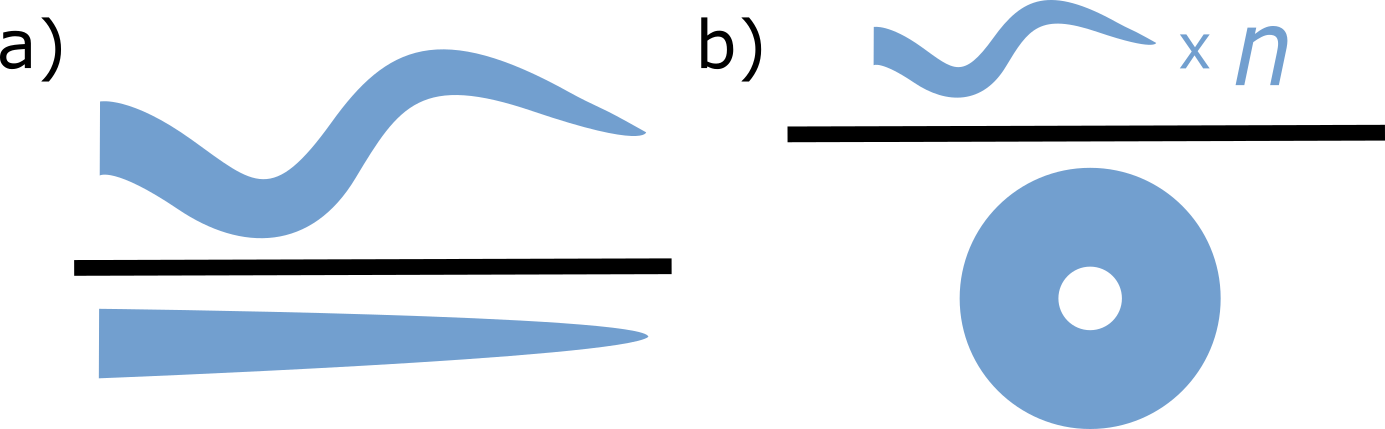
\includegraphics[width=\columnwidth]{figs/indices.png}
    \caption{Serpentine flexures are described by two design indices. a) the serpentine factor represents the sinuosity of the flexure and is calculated as serpentine area divided by the nominal straight flexure area. b) the density factor indicates the compactness of the flexures within the spring, dividing the combined area of all flexures by the total occupiable area.}
    \label{fig:indices}
\end{figure}
\section{HARDWARE VALIDATION OF SPRING DESIGN FRAMEWORK}
To demonstrate the efficacy of our design framework, we designed, manufactured, and empirically evaluated two springs with identical desired stiffness properties, but differing geometries (see Fig.~\ref{fig:main_design}). One spring was designed with straight flexures, while the other was designed with serpentine flexures. (Table~\ref{table:spring_params}). All other geometric constraints and material properties were equivalent, with the material selection being hardened SS420, a target spring rate of 150 Nm/rad, 24 flexures, a 4.5 mm spring thickness, and identical outer radii (33.5 mm). The intentional difference in serpentine factor was selected to demonstrate the range of motion (and thus energy storage) benefit of designing serpentine flexures.

% spring, spring rate (des, exp), max deflection/torque (des, exp), radius, weight
\begin{table}[h!]
    
    \caption{Design parameters and expected properties of both tested springs.}
    \centering
    % \begin{tabular}{ p{.7cm} p{.7cm} p{.7cm} p{.7cm} p{.7cm} p{.7cm} p{.7cm} }
    \begin{tabular}{c c c c c c c}
    \hline
    \multirow{3}{3em}{\centering\textbf{Spring Design}} & \multirow{3}{4em}{\centering\textbf{Spring Rate (Nm/rad)}} & \multirow{3}{4.5em}{\centering\textbf{Desired Deflection (rad)}} & \multirow{3}{2em}{\centering\textbf{Mass (g)}} & \multirow{3}{3em}{\centering\textbf{Serp. Factor}} & \multirow{3}{3em}{\centering\textbf{Density Factor}}\\ 
    & & & & & & \\
    & & & & & & \\
    \hline
    Straight & 150 & 0.241 & 57.3 & 1.00 & 0.39\\
    Serpentine & 150 & 0.262 & 71.0 & 1.14 & 0.47\\
    \hline
    \end{tabular}
    \label{table:spring_params}
\end{table}

\subsection{Serpentine Spring Design}
The practical implementation of designing serpentine flexures is nontrivial. Specifically, the analysis performed in Section II provides only two constraints on the serpentine geometry (planar flexure area and the taper), thus leaving the high-dimensional design problem unconstrained. To narrow the design space for these flexures, we intentionally designed springs that (1) originate and terminate along the same axis, (2) distribute area evenly across that axis (Fig.~\ref{fig:spring_diag}), (3) avoid sharp bends, and (4) do not intersect with neighboring flexures. Even with these additional design considerations, there exist several viable spring geometries; thus, for the physical serpentine test spring, we selected one of many satisfactory flexure designs.


\subsection{Methods}
\begin{figure}[b!]
    \centering
    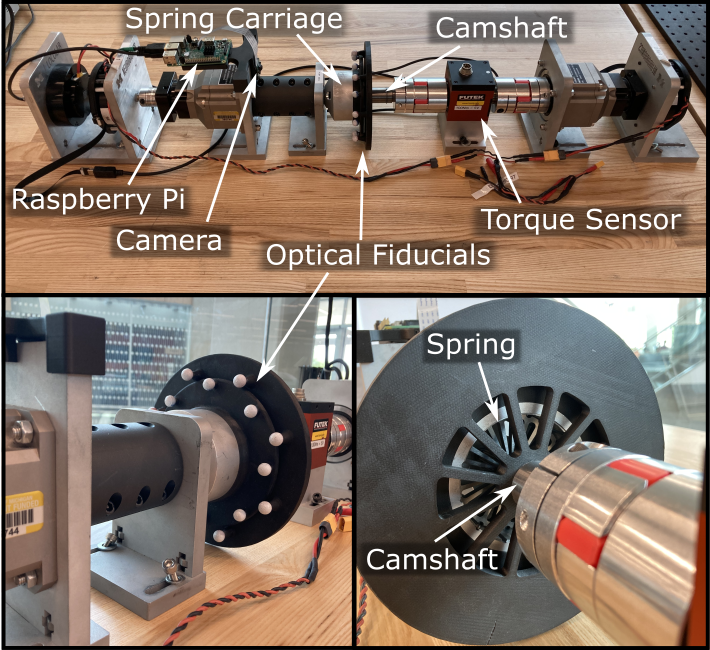
\includegraphics[width=\columnwidth]{figs/testbed.png}
    \caption{Custom dynamometry testbed used to evaluate spring performance.}
    \label{fig:testbed}
\end{figure}
We developed our experimental protocol to accurately characterize the test springs and thus validate the design approach. The benchtop testbed (Fig.~\ref{fig:testbed}) loaded each spring using two opposing actuators, while simultaneously measuring spring deflection and applied torque. Dowel rods were used to hold the springs inside a custom spring carriage and oppose the applied torques. We measured torque with a contactless sensor (TRS605, Futek, Irvine CA) in series with the spring assembly, and the sensor output an analog voltage that was sampled by a 16-bit analog-to-digital converter at 265 Hz. Rotation was induced by identical brushless DC actuators (ActPack, Dephy Inc, Maynard MA), each coupled to a transmission (50:1 PL2090-050, Boston Gear, Boston MA), and the motors were driven in position control using a microprocessor (RPi 3 Model B+, Raspberry Pi Foundation, Cambridge UK). Although both motors include encoders, we elected to measure spring deflection directly to ensure that the data described spring compliance and not the compliance of the entire dynamometry system.

\begin{figure}[t!]
    \centering
    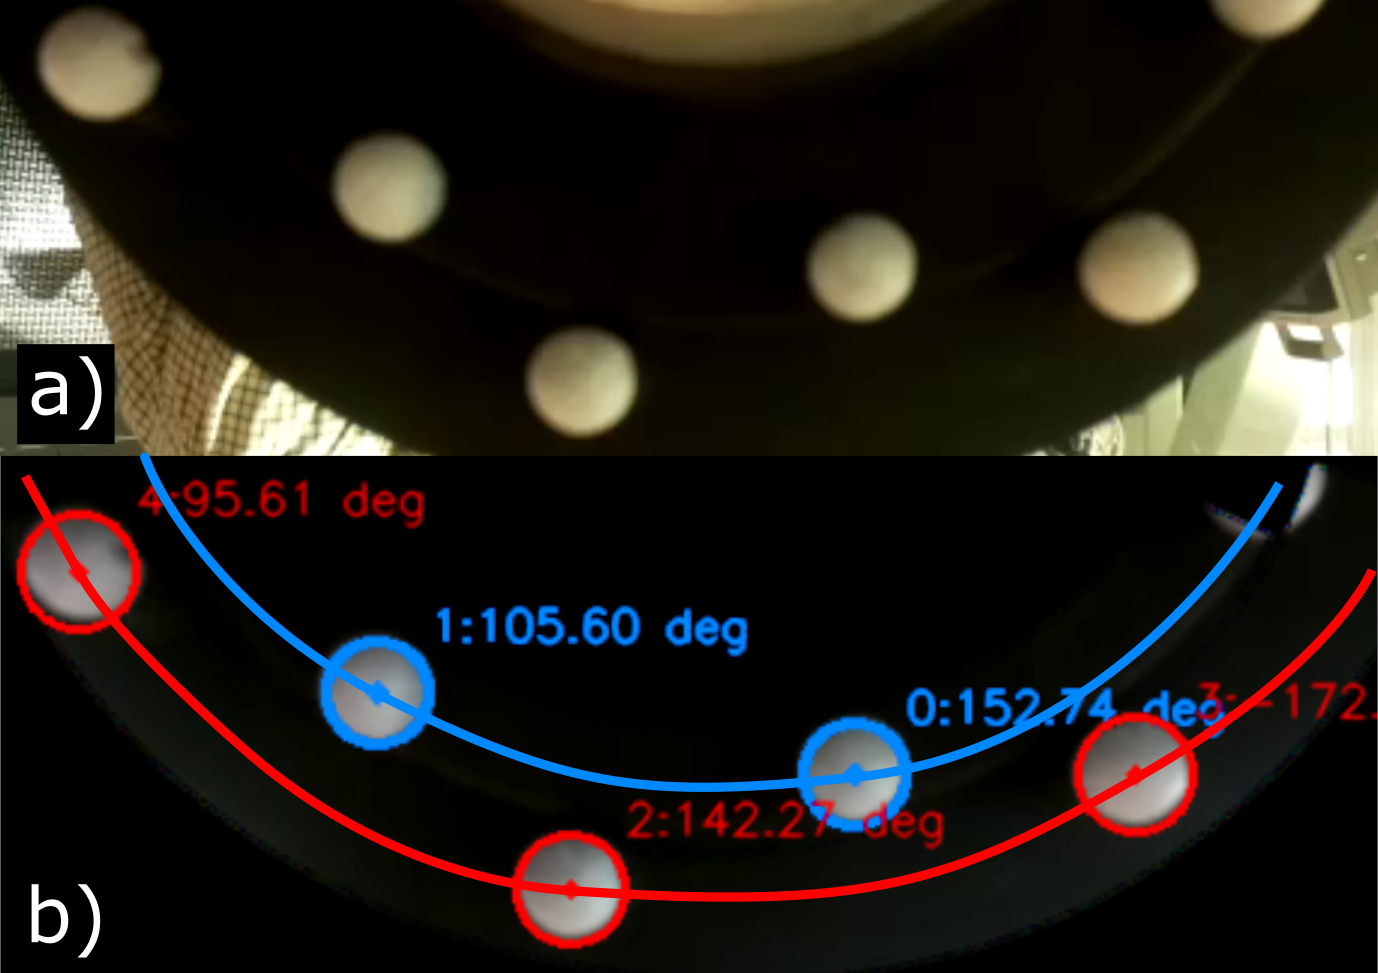
\includegraphics[width=\columnwidth]{figs/fiducial_fig.png}
    \caption{By tracking optical fiducials with a camera, we were able to measure true deflection of the springs. a) raw image from camera, b) processed version of the image with masks applied and fiducials being tracked.}
    \label{fig:fiducial}
\end{figure}

To measure spring deflection without the deflection of the transmission or testbed parts, we implemented a custom optical encoder and image processing algorithm to measure deflection of the spring only. The optical encoder consisted of two arrays of optical fiducials: one rigidly mounted to shaft with the other mounted to the spring carriage (Fig.~\ref{fig:testbed}). By tracking these fiducials (RPi Camera Module 2, Raspberry Pi Foundation, Cambridge UK) we recorded deflection at the spring interface, and the video was processed off-line to measure relative rotation (Fig.~\ref{fig:fiducial}). Custom filter masks focused the image processing on the two arcs containing fiducials. After masking, we used OpenCV \cite{opencv_library} to track the fiducials in the plane of the image (Fig.~\ref{fig:fiducial}b). We calculated incremental displacement of the spring-side and camshaft-side fiducials using best-fit ellipses obtained through calibration. To obtain the displacement of the spring, we simply subtracted spring-side angle from the shaft-side angle. As validation of the measurement, deflection of the optical fiducials closely tracked the motor encoders during unloaded motion of the testbed ($y=\text{0.9998}x-\text{0.0709 deg}$).

In testing the springs, we thoroughly traversed their respective expected operating deflection ranges. For each spring, we prescribed several setpoint deflection angles: two degrees, six degrees, ten degrees and then one-degree steps until well past the designed deflection limit. The setpoints were commanded in increasing magnitude to ensure that any yield or catastrophic failure would be preceded by valid measures of spring torque and deflection. As the setpoint magnitude increased, we decreased the step change to 1 degree for the same purpose of logging data before failure. For each setpoint, we started a test with the spring at zero deflection, ramped up to the positive value, ramped back to zero, ramped to the negative value, and then ramped back to zero, with each ramp lasting five seconds. During each test, we measured torque in the shaft with the contactless sensor and recorded high-definition video of the optical fiducials to enable accurate off-line deflection measurements. With torque and deflection measurements from the testing, we determined the torque-angle relationship of each spring.

\subsection{Results}

The measured spring behavior closely matched the desired performance. Notably, both springs achieved their designed deflection limits without signs of failure (Fig.~\ref{fig:lin_springrates}). Furthermore, the measured spring rates closely matched the target values (Table~\ref{table:linear_spring_rates}). As expected, the testing also measured the energy loss due to hysteresis during the loading and unloading process. At designed deflection (as depicted) the percent energy loss is approximately 10 percent (Straight: 9.72\%, Serpentine: 12.0\%); however, at smaller deflections of nine degrees, those percentages are dramatically lower (Straight: 0.41\%, Serpentine: 1.08\%).

The measured energy density and specific energy of the springs are promising when compared to the literature, and align with our predictions. Energy storage was calculated using the designed deflection and the measured average stiffness coefficient for each spring (Table~\ref{table:linear_spring_rates}), resulting in 4.53 J and 5.47 J for the straight and serpentine springs, respectively. Dividing by mass and enclosed volume yields 79.0 J/kg and 0.285 J/cm$^{3}$ for the straight spring and 77.0 J/kg and 0.345 J/cm$^{3}$ for the serpentine spring. Thus, when compared to the straight spring, the serpentine spring achieves significantly higher energy density and maximum deflection while maintaining similar specific energy.

\begin{figure}[b!]
    \centering
    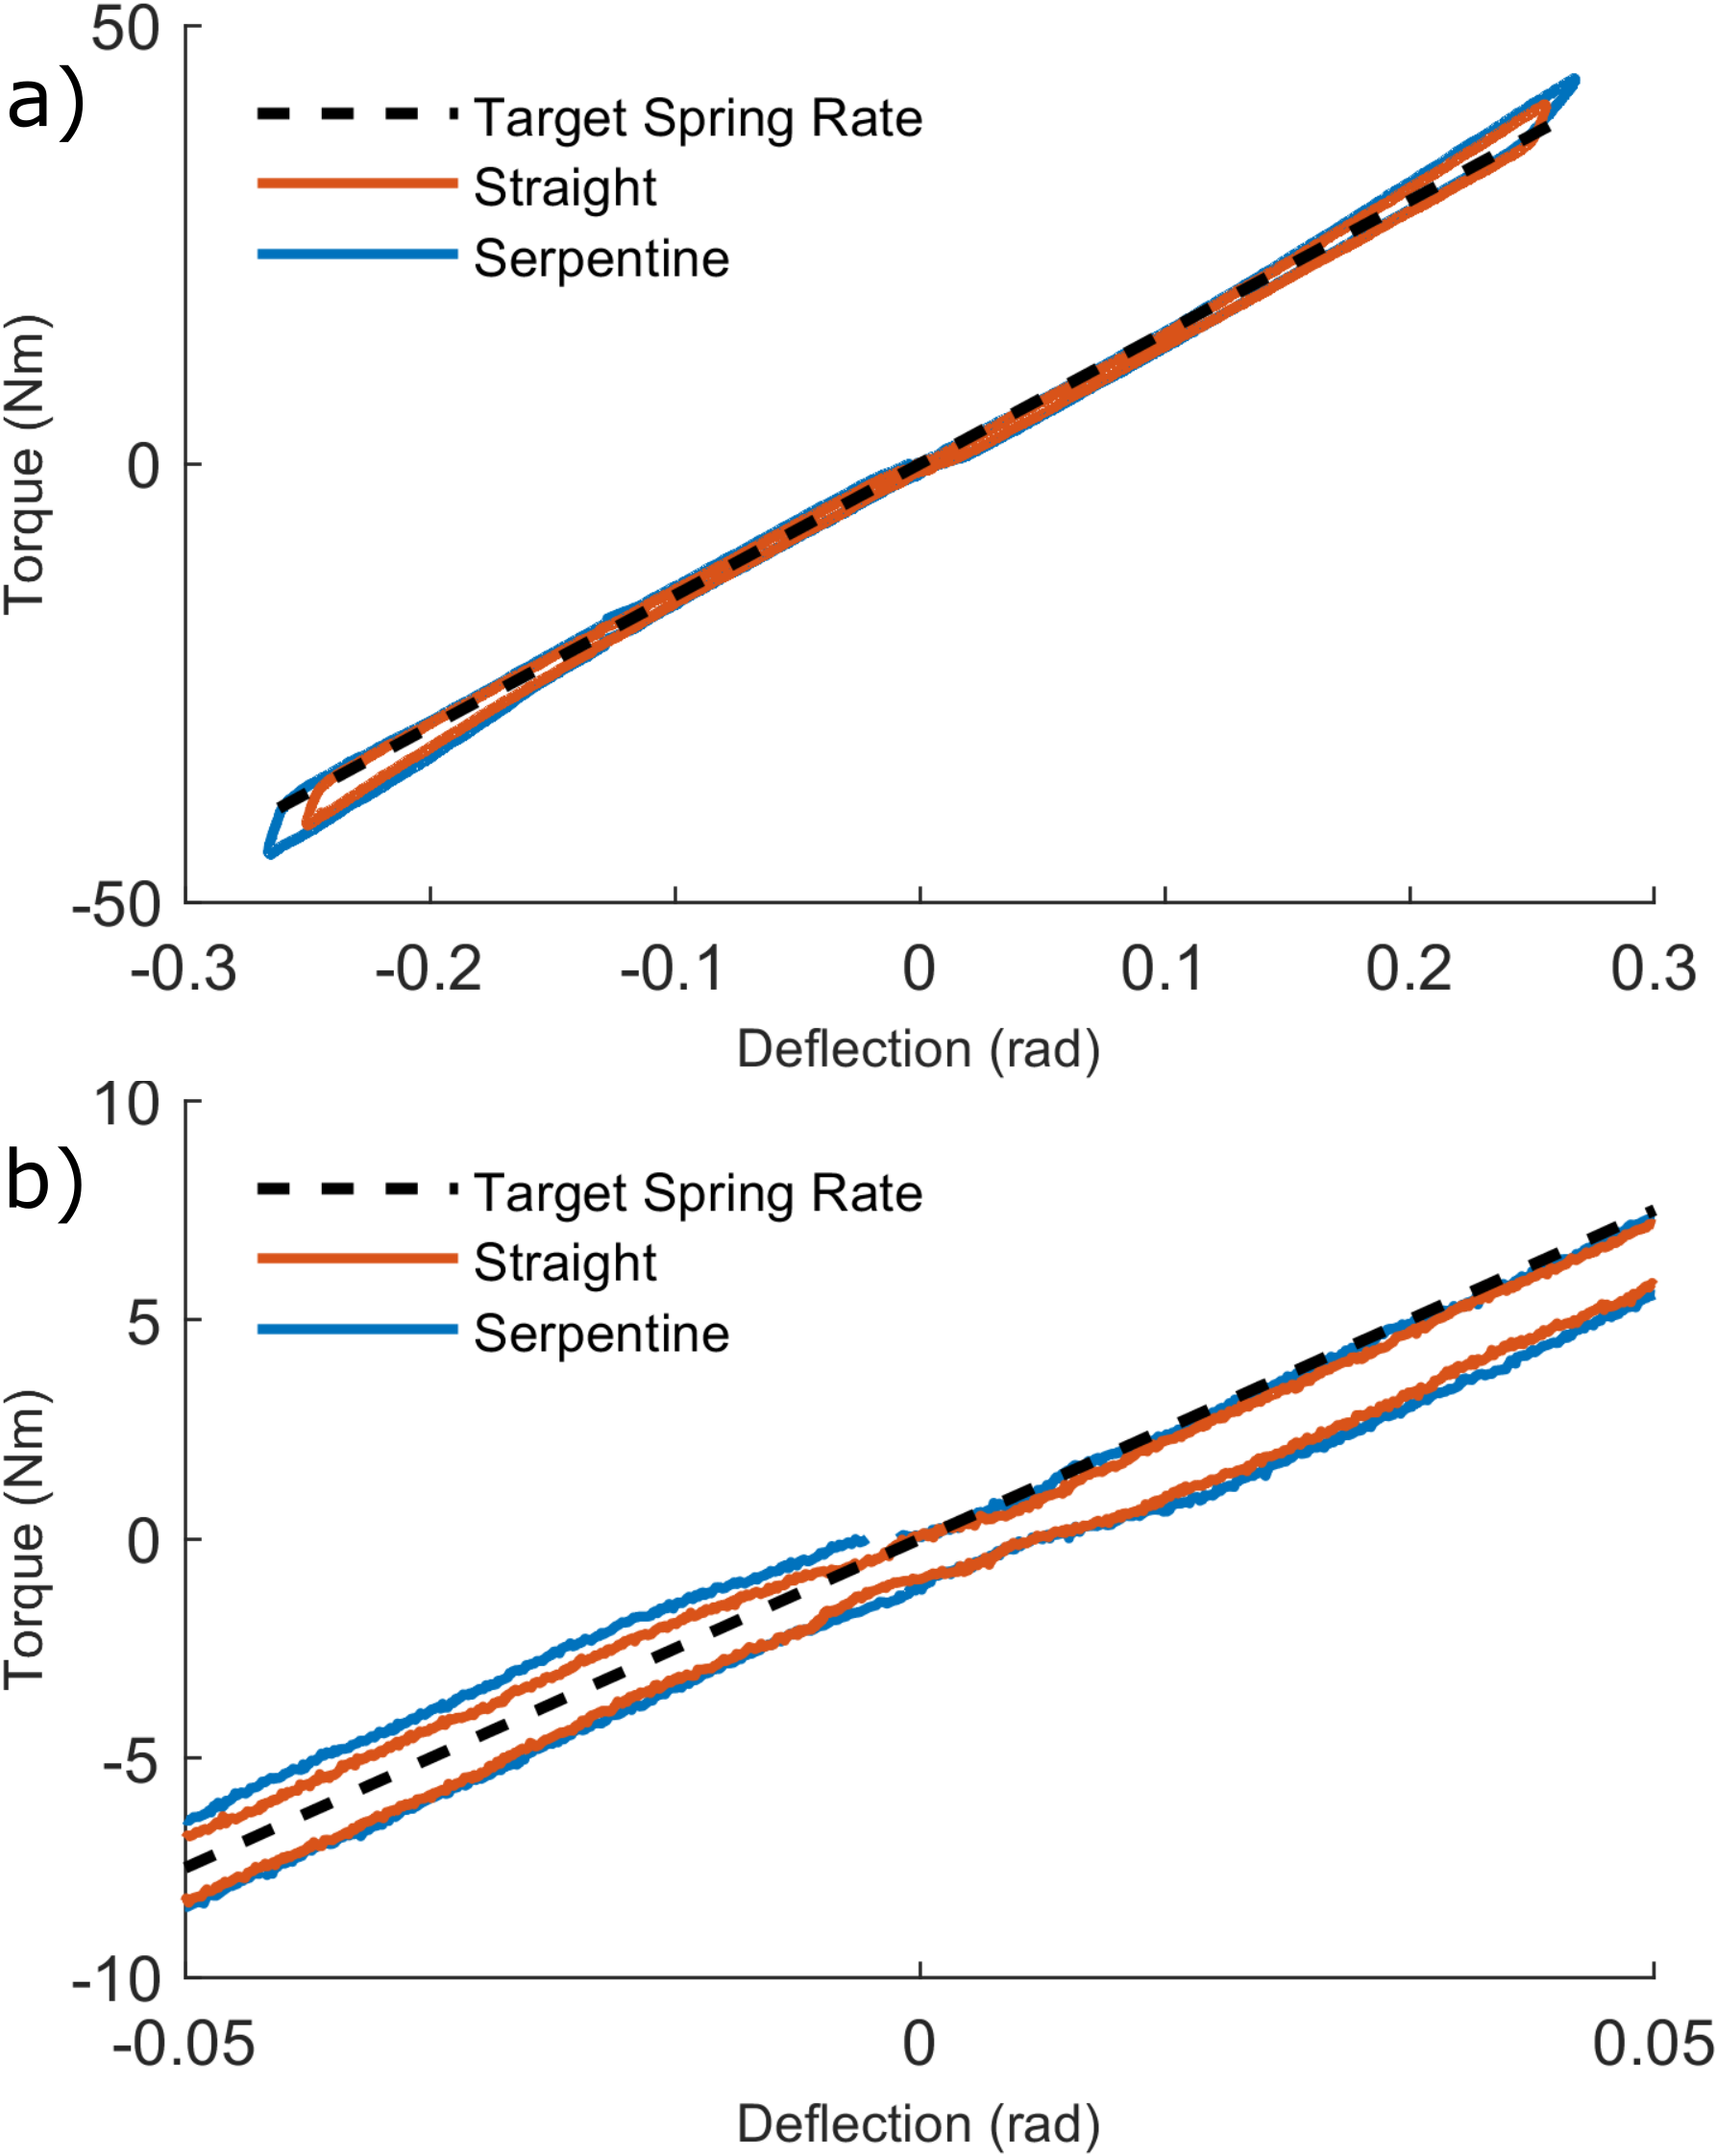
\includegraphics[width=\columnwidth]{figs/spring_plots.png}
    \caption{a) Measured stiffness profiles of both springs over their respective operable range. For reference, the target spring rate of 150 Nm/rad is also displayed. b) Magnified view around zero torque and deflection, which can be used to understand the backlash observed in the spring prototypes.}
    \label{fig:lin_springrates}
\end{figure}

\begin{table}[t]
    \caption{Spring properties in positive and negative torque regimes.}
    \centering
    \begin{tabular}{ c c c c c c c c  }
    \hline
    \multirow{3}{3em}{\textbf{Spring Design}} & \multicolumn{6}{c}{\textbf{Spring Stiffness Coefficient (Nm/rad)}} & \multirow{3}{1.5em}{\centering\textbf{Error (\%)}}\\
    & \multirow{2}{*}{\textbf{Des.}} & \multicolumn{2}{c}{\textbf{Loading}} & \multicolumn{2}{c}{\textbf{Unloading}} & \multirow{2}{1.5em}{\textbf{Avg.}} & \\ 
    & & \textbf{Pos.} & \textbf{Neg.} & \textbf{Pos.} & \textbf{Neg.} & &\\ 
    \hline
    Straight & 150 & 159.6 & 161.8 & 150.3 & 152.0 & 155.9 & 3.9\\
    Serpentine & 150 & 165.4 & 165.1 & 155.3 & 151.5 & 159.3 & 6.2\\
    \hline
    \end{tabular}
    \label{table:linear_spring_rates}
\end{table}

\section{DISCUSSION}
\subsection{Contributions}
%% Highlight main takeaways

    %% Recap paper --> main takeaway is new design
    Elastic elements are a critical aspect of many robotic systems, especially those that operate in close proximity with humans. In this paper, we presented the design and preliminary validation of a novel spring geometry. The motivation of our exploration was to design a sufficiently compact and lightweight spring to enable integration in a robotic prosthesis with no additional required volume \cite{AzocarRouse2020}. Our design framework radically deviates from conventional designs, comprising a circular array of tapered cantilever flexures in contact with a gear-like camshaft (Fig.~\ref{fig:main_design}).

    This new spring architecture enables the addition of series elasticity to robotic systems without any added volume. As explained previously, with intentional design, the compact spring can be housed within common transmission components, such as within the output pulley of a timing belt transmission used in \cite{AzocarRouse2020}. The spring also outperforms the current literature with respect to specific energy \cite{DossantosCurinSiqueira2017CEP,CarpinoEA2012JMD,GeorgievBurdick2017IROS,TsagarakisLaffranchiVanderborghtCaldwell2009ICRA,Stienen2010TBME,AccotoEA2013IJARS,HerodotouWang2019ICORR,WangMeijnekeVanderkooij2013ICORR,KnoxSchmiedeler2009JMD,LagodaEA2010ICBRB}, meaning that it adds a small amount of mass considering the magnitude of energy that can be stored. Coupled together in one design, these attributes enable the use of SEAs in robots that are constrained by size or mass. The unique combination of low stiffness and larger deflections possible in our spring architecture makes it particularly desirable in SEA applications, as it may enable improved torque-sensing resolution.

    %% Model = Physical system --> quick adoption
    Our preliminary validation demonstrates the accuracy of our modeling and design. The desired stiffness of the designed springs was 150 Nm/rad, and the measured error was 4.6\% (Tab.~\ref{table:linear_spring_rates}). We made a number of assumptions in our design framework and the relative accuracy of our approach demonstrates the assumptions were appropriate. The agreement between our model and empirical results highlights the ability for future researchers to use our approach to develop compact springs with high confidence in the physical design. Furthermore, the closed form solutions provided in our approach do not have the barriers of complicated derivations or iterative design methods using finite-element analysis.
    
    % Backlash, talk about it, quantify, talk about how balls made it better
    While our spring architecture consists of two separate parts, minimal backlash was observed. This is in contrast to previous versions of our springs where backlash was a concern. Backlash was mitigated by two strategies, namely adding a circular head to the flexure tooth tips that improved the mechanical interface with the gear-like cam shaft; in addition, we updated the material chosen for the spring from 7075-T6 aluminum to SS420 steel. When tested, the backlash was minimal, which can be observed directly in Fig.~\ref{fig:lin_springrates}b ($<\sim5$ mrad). 
    
    Lastly, our approach lays a foundation to explore several additional design variables within our spring architecture. For example, a formalized camshaft geometry would likely improve the correlation between the model and empirical results. Likewise, optimizing other design variables (see \eqref{eq:thetaexpression}) could yield significant increases in allowable deflections, and thus energy density.

\subsection{Limitations}
%% Limitations
    Our design framework produced accurate mechanics in a compact design, but more work is needed to reach the potential of this spring architecture. First, the hysteresis observed in the springs is moderate ($\sim$10\%). We expect that the loss is primarily due to the sliding contact between the flexures and the teeth of the camshaft, which would indicate that some hysteresis may be an unavoidable limitation of this approach; however, this study did not include any attempts to confirm the source of hysteresis or lessen its effects. Possible mitigation strategies could include lubrication of the faces in contact or improving their surface finish.
    
    Since springs are typically expected to endure many cycles of loading, accounting for fatigue is an important design consideration. For the springs tested in this study, fatigue was not considered, nor were cyclical loading tests performed to measure fatigue empirically. In future work, we will update the design framework to include the desired cycles to failure by adjusting the design stress specification within the framework.
    
\subsection{Broader Applicability}

    This spring design is promising and highly customizable, so possible applications are broad. The most significant area of impact would likely be in mobile robots that utilize SEAs, parallel elastic mechanisms, or other uses where compliance is beneficial; for example, humanoid robots, legged robots, serial-link manipulators, prosthetic limbs, and exoskeletons, among others. Alternatively, there are many modifications or further developments that could be pursued to make this design more broadly applicable. For example, the bending beam paradigm could be transformed to yield prismatic springs, which could be useful as a high-efficiency alternative to springs in series with linear actuators, or in mechanisms such as suspension systems. Another possibility is to implement series interconnections of the spring, enabling larger deflection limits \cite{CarpinoEA2012JMD}. Lastly, the under-constrained interface between the camshaft and the spring could be exploited to create a sliding clutch or variable spring-rate mechanism (\textit{e.g.} stiffening springs).

\section{CONCLUSION}
In this paper, we presented a novel spring design characterized by a ring of radially-extending tapered cantilever beams in contact with a gear-like camshaft. To our knowledge, this new approach yields the most energy-efficient springs to date. We tested the mechanics of two representative springs on a custom testbed to investigate the fidelity of our design framework. We believe this work increases the potential for incorporating series and parallel springs into lightweight and compact mechanisms.

% \addtolength{\textheight}{-12cm}   % This command serves to balance the column lengths
                                  % on the last page of the document manually. It shortens
                                  % the textheight of the last page by a suitable amount.
                                  % This command does not take effect until the next page
                                  % so it should come on the page before the last. Make
                                  % sure that you do not shorten the textheight too much.


% use section* for acknowledgment
% \section*{Acknowledgment}

\bibliographystyle{IEEEtran}
\bibliography{bib}
\end{document}
